\documentclass{article}

%
% Paket für Übersetzungen ins Deutsche
%
\usepackage[ngerman]{babel}

\usepackage{geometry}

\usepackage{pdfpages} 

%
% Pakete um Latin1 Zeichnensätze verwenden zu können und die dazu
% passenden Schriften.
%
\usepackage[utf8]{inputenc}
%\usepackage[T1]{fontenc}

%
% Paket zum Erweitern der Tabelleneigenschaften
%
\usepackage{array}

%
% Paket für schönere Tabellen
%
\usepackage{booktabs}

%
% Paket für Referenzen
%
\usepackage{prettyref}
\usepackage{titleref}

\usepackage{xcolor}

\usepackage{listings}
\definecolor{codegreen}{rgb}{0,0.6,0}
\definecolor{codegray}{rgb}{0.5,0.5,0.5}
\definecolor{codepurple}{rgb}{0.58,0,0.22}
\definecolor{backcolour}{rgb}{0.15,0.15,0.12}
 
\lstdefinestyle{mystyle}{
    backgroundcolor=\color{white},   
    commentstyle=\color{codegreen},
    keywordstyle=\color{codepurple},
    numberstyle=\tiny\color{codegray},
    stringstyle=\color{codepurple},
    basicstyle=\footnotesize,
    breakatwhitespace=false,         
    breaklines=true,                 
    captionpos=b,                    
    keepspaces=true,                 
    numbers=left,                    
    numbersep=5pt,                  
    showspaces=false,                
    showstringspaces=false,
    showtabs=false,                  
    tabsize=2
}
 
\lstset{style=mystyle}
%
% Paket um Grafiken einbetten zu können
%
\usepackage{graphicx}
\makeatletter
\def\ScaleIfNeeded{%
\ifdim\Gin@nat@width>\linewidth
\linewidth
\else
\Gin@nat@width
\fi
}
\makeatother


%
% Kopf und Fußzeilen
%
\usepackage{scrpage2}
\pagestyle{scrheadings}
% Inhalt bis Section rechts und Chapter links
\automark[section]{chapter}
% Mitte: leer
\chead{}

\usepackage[textfont=bf,singlelinecheck=true,justification=centering]{caption}
\DeclareCaptionLabelSeparator{linebreak}{\\}
\captionsetup{labelsep=linebreak}


%
% mathematische symbole aus dem AMS Paket.
%
\usepackage{amsmath}
\usepackage{amssymb}
\usepackage{nicefrac}

\usepackage{verbatim}

\usepackage{pifont}% http://ctan.org/pkg/pifont
\newcommand{\cmark}{\color{green}\ding{51}}%
\newcommand{\xmark}{\color{red}\ding{55}}%

\usepackage{pgfplots}
\pgfplotsset{
	major grid style={densely dotted,black!30},
	minor grid style={densely dotted,black!30},
    box plot/.style={
        /pgfplots/.cd,
        blue,
        only marks,
        mark=-,
        mark size=0em,
        /pgfplots/error bars/.cd,
        y dir=plus,
        y explicit,
    },
    other color/.style={
	    /pgfplots/.cd,
    	red
    },
    box plot box/.style={
        /pgfplots/error bars/draw error bar/.code 2 args={%
            \draw[gray,thick] ##1 |- ##2;
        },
        /pgfplots/table/.cd,
        y index=2,
        y error expr={\thisrowno{3}-\thisrowno{2}},
        /pgfplots/box plot
    },
    box plot top whisker/.style={
        /pgfplots/error bars/draw error bar/.code 2 args={%
            \pgfkeysgetvalue{/pgfplots/error bars/error mark}%
            {\pgfplotserrorbarsmark}%
            \pgfkeysgetvalue{/pgfplots/error bars/error mark options}%
            {\pgfplotserrorbarsmarkopts}%
            \path[gray,thick] ##1 |- ##2;
        },
        /pgfplots/table/.cd,
        y index=4,
        y error expr={\thisrowno{2}-\thisrowno{4}},
        /pgfplots/box plot
    },
    box plot bottom whisker/.style={
        /pgfplots/error bars/draw error bar/.code 2 args={%
            \pgfkeysgetvalue{/pgfplots/error bars/error mark}%
            {\pgfplotserrorbarsmark}%
            \pgfkeysgetvalue{/pgfplots/error bars/error mark options}%
            {\pgfplotserrorbarsmarkopts}%
            \path[gray,thick] ##1 |- ##2;
        },
        /pgfplots/table/.cd,
        y index=5,
        y error expr={\thisrowno{3}-\thisrowno{5}},
        /pgfplots/box plot
    },
    box plot median/.style={
        /pgfplots/box plot,
        /pgfplots/.cd,
        mark size=.4em,
        thick
    }
}

%
% zum Zeinen von Bäumen
%
\usepackage{fancybox}
\usepackage{tikz}
\usetikzlibrary{calc}

\usepackage{cite}

% Um algorithmen und Code schoen aussehen zu lassen
\usepackage{listings}
%\usepackage{algorithm,algorithmic}

%
% Paket um Textteile drehen zu können
%
\usepackage{rotating}

%
% Paket für Farben im PDF
%
\usepackage{color}

%
% Paket für Links innerhalb des PDF Dokuments
%
\definecolor{LinkColor}{rgb}{0,0,0.5}
\usepackage[
	pdftitle={Titel},									% Titel der Bachelorarbeit
	pdfauthor={Autor},									% Autor(en)
	pdfcreator={LaTeX, LaTeX with hyperref and KOMA-Script},	% Genutzte Programme
	pdfsubject={Betreff},			 					% Betreff
	pdfkeywords={Keywords}]{hyperref} 					% Keywords halt :-)
\hypersetup{colorlinks=true,								% Definition der Links im PDF File
	linkcolor=LinkColor,
	citecolor=LinkColor,
	filecolor=LinkColor,
	menucolor=LinkColor,
	urlcolor=LinkColor}

%
% Paket um LIstings sauber zu formatieren.
%
\usepackage{listings}
%
% Listing Definationen für PHP Code
%
\definecolor{lbcolor}{rgb}{0.85,0.85,0.85}
\lstset{language=[LaTeX]TeX,
	numbers=left,
	stepnumber=1,
	numbersep=5pt,
	numberstyle=\tiny,
	breaklines=true,
	breakautoindent=true,
	postbreak=\space,
	tabsize=2,
	basicstyle=\ttfamily\footnotesize,
	showspaces=false,
	showstringspaces=false,
	extendedchars=true,
	backgroundcolor=\color{lbcolor}}


%
% aller Bilder werden im Unterverzeichnis figures gesucht:
%
\graphicspath{{Bilder/}}

\usepackage[onehalfspacing]{setspace}

%
% Strukturiertiefe bis subsubsection{} möglich
%
\setcounter{secnumdepth}{3}

%
% Dargestellte Strukturiertiefe im Inhaltsverzeichnis
%
\setcounter{tocdepth}{3}

%
% Literaturverzeichnis-Stil
%
\bibliographystyle{alpha}

\usepackage{anysize}
\begin{document}

\def\nicefrac#1#2{ \raise.5ex\hbox{$#1$}%
 \kern-.1em/\kern-.15em%
  \lower.25ex\hbox{$#2$}}

\title{GPU-Implementierung des RSH-Extraktors}
\author{Dominik Stamm, Markus Dollinger}
\maketitle

\section{DerRSH-Extraktor}
\section{Anforderungen an den GPU Algorithmus}

Aufgrund der unterschiedlichen Architektur von CPUs und GPUs, kann der RSH-Extraktor nicht einfach portiert werden, sondern muss, mit Fokus auf die Vor- und Nachteile einer GPU, neu entwickelt werden. Eine CPU hat - verglichen mit einer GPU - sehr wenige parallele Ausf"uhrungseinheiten, daf"ur einen gr"o"seren Befehlssatz und deutlich mehr Steuerlogik, wodurch CPUs ihre Ausf"uhrungsressourcen deutlich besser auslasten k"onnen. Somit sind CPUs besser geeignet f"ur Berechnungen die eine geringe Datenparallelit"at haben. GPUs sind aufgrund ihrer geringen Steuerlogik und ihrer hohen Anzahl an parallelen Ausf"uhrungseinheiten f"ur Berechnungen geeignet die eine hohe Datenparallelit"at haben. Die Effizienz des Extraktionsprozesses h"angt deswegen sehr stark von der F"ahigkeit ab, die n"otigen Berechnungen so gut wie m"oglich zu parallelisieren. 

Die unterschiedlichen Cache-Hierarchien und -Typen stellen ebenfalls eine Herausforderung dar. Um das volle Potential einer GPU auszunutzen reicht es nicht einfach nur massiv zu parallelisieren, sondern es muss beachtet werden, auf welche Speicherbereiche zugegriffen werden kann. Eine GPU bietet im Allgemeinen drei Speicherbereiche:
\begin{itemize}
	\item privater Speicher: Nur ein Thread hat zugriff (sehr schnell)
	\item lokaler Speicher: Threads einer Arbeitsgruppe haben zugriff (schnell)
	\item globaler Speicher: Alle Threads haben zugriff (langsam)
\end{itemize}
Dar"uber hinaus ist es nicht m"oglich Threads global zu synchronisieren. F"ur Berechnungen die keinerlei Abh"angigkeiten haben, ist das kein Problem. Bei der Multiplikation zweier gro"ser Zahlen kann z.B. die Multiplikation der einzelnen Bl"ocke komplett parallel nach der Schulmethode durchgef"uhrt werden. Die anschlie"senden Additionen k"onnen jedoch nicht ohne weiteres parallelisiert werden, da Datenabh"angigkeiten bestehen. Es ist m"oglich die Additionen in $\log(N)$ Schritten durchzuf"uhren, indem jede Ebene des Additionsbaumes komplett parallelisiert wird (Siehe \cite{haque2012plain} Kapitel 3 f"ur eine detaillierte Erkl"arung), allerdings m"ussen alle Operationen einer Ebene fertig sein, bevor zur n"achsten übergegangenen werden kann, d.h. am Ende jeder Ebene muss synchronisiert werden. Threads auf der GPU k"onnen nur lokal synchronisiert werden, das bedeutet, dass bei diesem Beispiel nicht das komplette Potential der GPU ausgereizt werden kann, sondern maximal das Potential einer Arbeitsgruppe, wodurch Einschr"ankungen entstehen k"onnen.

Um den Implementierungsaufwand zu minimieren, wurde nach bereits existierenden Algorithmen in Form von Bibliotheken oder "ahnlichem gesucht, welche die ben"otigten mathematischen Berechnungen bereits implementieren. Ein "Uberblick "uber die gefundenen Bibliotheken wird im n"achsten Kapitel gegeben.
\section{Getestete Bibliotheken}
\label{Bibliotheken}

Der RSH-Extraktor hat mathematische Anforderungen, die "uber die F"ahigkeiten der in Hardware verf"ugbaren Arithmetik hinausgehen. Um den Extraktor auf einen Grafikprozessor portieren zu k"onnen, m"ussen folgende Operationen unterst"utzt werden:
\begin{itemize}
	\item Multiplizieren und Evaluieren von Polynomen "uber $GF(2^n)$
	\item Rechnen mit sehr gro"sen Zahlen, da Koeffizienten mit mehr als 1000 Bit entstehen k"onnen
\end{itemize}

Um GPUs f"ur Berechnungen zu nutzen gibt es verschiedene APIs. Die CUDA-API ist eine von Nvidia entwickelte Programmier-Technik die es erm"oglicht Berechnungen auf die Hauseigenen GPUs auszulagern. OpenCL ist ein von der Khronos Group initiierter offener Standard um Berechnungen auf GPUs durchzuf"uhren. Dabei gibt es keine Beschr"ankung auf einen spezifischen GPU-Hersteller und w"are deshalb CUDA vorzuziehen. Eine dritte M"oglichkeit ist DirectCompute, eine in die DirectX-API integrierte Schnittstelle und damit auf Windows-Plattformen beschr"ankt.

Eine Recherche nach einer geeigneten Basis f"uhrte zu CUDA-Bibliotheken. Eine OpenCL-Bibliothek war zum Zeitpunkt der Recherche nicht verf"ugbar.

\subsection{CUMODP}
Die Cuda Modular Polyomial (CUMODP) Bibliothek implementiert arithmetische Operationen f"ur dicht besetzte Matrizen und dicht besetzte Koeffizientenvektoren von Polynomen. Der Fokus liegt bei ganzzahligen Koeffizienten und die Bibliothek steht unter der GPL.
Allerdings existiert keine Unterst"utzung f"ur Zahlen beliebiger L"ange und keine Arithmetik "uber $GF(2^n)$, sodass CUMODP den Anforderungen nicht gen"ugt.

\subsection{CUMP}
Die CUDA Multiple Precision Arithmetic (CUMP) Bibliothek basiert auf der GNU MP (GMP) Bibliothek und implementiert Gleitkommaarithmetik mit beliebiger Genauigkeit. Die Bibliothek kann als Ersatz f"ur GMP verwendet werden, um die Arithmetik von der CPU auf die GPU zu verlagern. Die Bibliothek steht ebenfalls unter der GPL.
CUMP bietet zwar Unterst"utzung f"ur Zahlen beliebiger L"ange, jedoch keine M"oglichkeit zur Evaluierung von Polynomen und auch keine Arithmetik "uber $GF(2^n)$. Dadurch gen"ugt auch CUMP nicht den Anforderungen.

\subsection{GARPREC}
Die GARPREC Bibliothek unterst"utzt ebenfalls Gleitkommaarithmetik mit beliebiger Genauigkeit, jedoch ebenfalls keine M"oglichkeit zur Evaluierung von Polynomen und auch keine Arithmetik "uber $GF(2^n)$.
GARPEC steht ebenfalls unter der GPL.

\subsection{GPUMP}
Die GPUMP Bibliothek implementiert Ganzzahlarithmetik mit beliebiger Genauigkeit. Der Fokus liegt bei der Verwendung in Public Key Kryptographie (PKK) Verfahren. Durch das Fehlen der Arithmetik "uber die ben"otigten Erweiterungsfelder sowie die M"oglichkeit zur Polynomevaluierung ist auch diese Bibliothek nicht geeignet. Der Quellcode der Bibliothek wird nicht als Download angeboten, sondern war nur auf Anfrage zu erhalten. Dar"uber hinaus f"uhrt die Absenz einer Lizenz zu einer rechtlich unklaren Situation.

\begin{table}
\centering
\begin{tabular}{lccc}
\toprule
		Bibliothek & gro"se Zahlen & $GF(2^n)$-Arithmetik & Polynomevaluierung \\
\midrule
		CUMODP	& \xmark & \xmark & \cmark \\
		CUMP	& \cmark & \xmark & \xmark \\
		GARPREC	& \cmark & \xmark & \xmark \\
		GPUMP	& \cmark & \xmark & \xmark \\
\bottomrule
\end{tabular}
	\caption{Gegen"uberstellung der Bibliotheken}
	\label{table:vergleichBibliotheken}
\end{table}

\section{Implementierung}

Da keine der gefundenen Bibliotheken alle Anforderungen erfüllt, musste eine eigene Implementierung entwickelt werden, die alle ben"otigten mathematischen Berechnungen durchführen kann.

\subsection{Parallele Polynevaluierung}
Der Standardalgorithmus für die Polynomevaluierung auf CPUs ist das \textit{Horner-Schema}, da dies die minimale Anzahl an Additionen und Multiplikationen benötigt\cite{Ostrowski:1954}\cite{Pan:1966}. Leider ist beim Horner-Schema jeder Berechnungsschritt abhängig vom Zwischenergebnis des letztes Schrittes, was einer Parallelisierung des Algorithmus im Wege steht.\newline
Ein weiteres Verwahren zur Polynomevaluierung ist das \textit{Estrin-Schema}\cite{EstrinsScheme}. Das Estrin-Schema versucht die schlechte Parallelisierbarkeit des Horner-Schemas zu eliminieren, indem das zu evaluierende Polynom so in Teilausdrücke aufgeteilt wird, dass einzelne Teile der Formel parallel abgearbeitet werden. Dieses Verfahren kommt zwar im Gegensatz zum Horner-Schema mehr mit der minimalen Anzahl von Additionen und Multiplikationen aus, dies wird zu Gunsten der besseren Parallelisierbarkeit allerdings akzeptiert.\newline
Formel \eqref{estrin} zeigt, wie beispielsweise ein Polynom vom Grad 4 mit Hilfe des Estrin-Schemas aufgelöst werden kann.
\begin{equation}\label{estrin}
P(x) = a_4x^4 + a_3x^3 + a_2x^2 + a_1x + a_0 = a_4x^4 + (a_2+a_3x)x^2 + (a_0+a_1x)
\end{equation}

Leider ist auch das Estrin-Schema nicht optimal auf einer GPU parallelisierbar, da zum einen initial jedes Polynom in Abhängigkeit seines Grades in Gruppen zerlegt werden muss und zum anderen die notwendigen Potenzen von $x$ berechnet werden müssen, bevor der Algorithmus angewandt werden kann. Wenn allerdings alle Potenzen von $x$ initial berechnet werden müssen und im weiteren Verlauf zur Verfügung stehen, ist im Kontext der GPU Programmierung der effektivste Weg das Polynom auszuwerten, indem alle Koeffizienten mit den nötigen Potenzen von $x$ multipliziert werden. Für diesen Schritt kann je Multiplikation ein Kernelthread verwendet werden, wodurch die Berechnung bei einer ausreichend großen Anzahl an Threads in einem Zyklus abgearbeitet werden kann. 
Der verbleibende Schritt, in dem die Teilergebnisse zu einem Gesamtergebnis aufsummiert werden, kann zudem mit einer Laufzeit von $O(\log(n))$ abgearbeitet werden, wie später gezeigt wird.
Dadurch ergibt sich bei berechneten Werten der Potenzen $x^0 \dots x^{n-1}$ von $x$ und einer guten Parallelisierung für die Auswertung des Polynoms in Formel \eqref{estrin} eine Laufzeit von $O(\log(n)+1) = O(\log(n))$, wohingegen das Estrin-Schema bei einem Polynom vom Grad 4 insgesamt 4 Multiplikationen und 4 Additionen benötigt, was einer Laufzeit von $O(2n)$ entspricht. Durch Parallelisierung des Estrin-Schemas erhält man etwa eine Laufzeit von $O(n)$, dies ist allerdings immer noch schlechter als die Laufzeit von $O(\log(n))$ der Eigenimplementierung. Aufgrund der Form der Teilausdrücke des Estrin-Schemas wäre es zudem möglich, diese durch spezielle \textit{Multiply-Accumulate} Befehle berechnen zu lassen, was die Laufzeit weiter reduzieren würde. Aufgrund des nötigen Supports großer Zahlen durch die GPU ist dies für den gegebenen Anwendungsfall allerdings auch nicht möglich. Dadurch wurden sowohl das Horner-Schema als auch das Estrin-Schema nicht weiter in Betracht gezogen.\par

Der erste Schritt bei der Entwicklung eines Algorithmus musste somit sein, alle notwendigen Potenzen von $x$ effizient auf einer GPU berechnen zu können. Als Basis wurde der in \cite{Harris:2014} beschriebene \textsc{Prefix Sum Scan Algorithmus} verwendet. Dieses Verfahren bildet aus einer Folge von Zahlen deren Partialsummen. Beispielsweise ergibt sich die Präfixsumme der Zahlen $a_0$, $a_1$, $a_2$, $a_3$ aus aus den Partialsummen
\begin{align}\label{prefix_sum}
\begin{split}
s_0 &= a_0 \\
s_1 &= a_0 + a_1 \\
s_2 &= a_0 + a_1 + a_2 \\
s_3 &= a_0 + a_1 + a_2 + a_3
\end{split}
\end{align}

Durch die Gleichungen \eqref{prefix_sum} kann man bereits erkennen, dass dieser Algorithmus leicht auf die Berechnung der Potenzen $x^0 \dots x^{n-1}$ von $x$ adaptiert werden kann. Um dies zu erreichen, werden als Berechnungsrundlage nicht mehr unterschiedliche Zahlen, sondern lediglich $x$ verwendet. Zudem muss die Addition durch eine Multiplikation ersetzt werden. Dadurch ergeben sich die 4 Partialsummen in \eqref{prefix_sum} zu
\begin{align}\label{prefix_x_prod}
\begin{split}
s_0 &= x = x^1 \\
s_1 &= x \cdot x = x^2 \\
s_2 &= x \cdot x \cdot x = x^3 \\
s_3 &= x \cdot x \cdot x \cdot x = x^4
\end{split}
\end{align}
Wegen der Analogie zur Präfixsumme und der verwendeten Multiplikation wird dieses Verfahren im weiteren Verlauf als Präfixprodukt bezeichnet.

Die Implementierung des Präfixproduktes erfolgt mittels eines Binärbaums, wie es auch in \cite{Harris:2014} für die Präfixsumme beschrieben wird. Initial müssen dazu die einzelnen Blätter des Baumes mit der zu potenzierenden Variablen $x$ gefüllt werden. Dabei muss beachtet werden, dass das Ergebnis auch das Partialprodukt $x^0 = 1$ enthält, wodurch die Anzahl der Blätter des Baumes gleich der Anzahl der Koeffizienten des Ausgangspolynoms entsprechen muss. Zudem bedeutet die Verwendung eines Binärbaums, dass die Anzahl der Blätter eine Potenz von $2$ sein muss, wodurch beispielsweise bei $50$ Koeffizienten insgesamt $64$ Blätter zu zu erstellen sind. Im weiteren Verlauf wird die Anzahl der Blätter als $l$ und die nächst größere Potenz von $2$ als $lu$ bezeichnet, wobei gilt $lu=2^u \ge l \ge l^{u-1}$.\newline

Es sei an dieser Stelle angemerkt, dass bei der hier beschriebenen Implementierung der höchste Koeffizient immer den kleinsten Index besitzt. Aus diesem Grund wird auch vom Präfixprodukt ein Ergebnisarray bestehend aus allen Potenzen von $x$ erstellt, wobei der Grad der Potenz von $x$ mit zunehmendem Index abnimmt.\newline

Die Berechnung des Präfixproduktes kann in zwei Schritte, den \textit{Reduce-} und den \textit{Down-Sweep-Step}, aufgeteilt werden. Um die Arbeitsweise des Algorithmus zu beschreiben, sei das zu evaluierende Ausgangspolynom von Grad $d = 5$, bestehend aus $l = 6$ Koeffizienten:
$$P(x) = a_5x^5 + a_4x^4 + a_3x^3 + a_2x^2 + a_1x +a_0$$ 
Für den Reduce-Step müssen somit $lu = 2^3 = 8$ Blätter erzeugt werden, was in Abb. \ref{fig:reduce_step} auf unterster Ebene dargestellt ist. 
Beginnend mit einer Schrittweite von $1$ werden im Iterationsschritt $i=0$ die zwei aufeinanderfolgenden Zelleninhalte der Blätter multipliziert. 
Anschließend wird die Schrittweite verdoppelt, wodurch im nächsten Iterationsschritt ($i=1$) die Elemente an Position $0$ und $2$ sowie $4$ und $6$ multipliziert werden.
Der Algorithmus terminiert, wenn die Schrittweite kleiner der Anzahl an Blättern $lu$ ist.
Das resultierende Array beinhaltet alle Potenzen $x^{2^i}$, mit $i=0 \dots \operatorname{ld}(lu)$. Da die Multiplikationen in jeder Ebene parallel durchgeführt werden können, ergibt sich bei optimaler Parallelisierung eine Laufzeit von $O(\log(lu))$, was bei dem in Abb. \ref{fig:reduce_step} dargestellten Array mit $8$ Elementen $3$ Iterationen entspricht. Zudem werden für $8$ Koeffizienten $4$ Cuda-Threads benötigt.\newline

\begin{figure}
\centering
\begin{tikzpicture}[level/.style={sibling distance=60mm/#1}]

\def\HEIGHT{1}
\def\WIDTH{1.5}

% leaves
\node (rect) at (0*\WIDTH,0) [draw,minimum width=\WIDTH cm,minimum height=\HEIGHT cm, fill=blue!30] (a0) {$x$};
\node (rect) at (1*\WIDTH,0) [draw,minimum width=\WIDTH cm,minimum height=\HEIGHT cm, fill=blue!30] (a1) {$x$};
\node (rect) at (2*\WIDTH,0) [draw,minimum width=\WIDTH cm,minimum height=\HEIGHT cm, fill=blue!30] (a2) {$x$};
\node (rect) at (3*\WIDTH,0) [draw,minimum width=\WIDTH cm,minimum height=\HEIGHT cm, fill=blue!30] (a3) {$x$};
\node (rect) at (4*\WIDTH,0) [draw,minimum width=\WIDTH cm,minimum height=\HEIGHT cm, fill=blue!30] (a4) {$x$};
\node (rect) at (5*\WIDTH,0) [draw,minimum width=\WIDTH cm,minimum height=\HEIGHT cm, fill=blue!30] (a5) {$x$};
\node (rect) at (6*\WIDTH,0) [draw,minimum width=\WIDTH cm,minimum height=\HEIGHT cm, fill=blue!30] (a6) {$x$};
\node (rect) at (7*\WIDTH,0) [draw,minimum width=\WIDTH cm,minimum height=\HEIGHT cm, fill=blue!30] (a7) {$x$};

\node (rect) at (0*\WIDTH,2) [draw,minimum width=\WIDTH cm,minimum height=\HEIGHT cm, fill=yellow!40, align=center] (b0) {$x^2$\\\scriptsize{(Thread 0)}};
\node (rect) at (1*\WIDTH,2) [draw,minimum width=\WIDTH cm,minimum height=\HEIGHT cm, fill=blue!30] (b1) {$x$};
\node (rect) at (2*\WIDTH,2) [draw,minimum width=\WIDTH cm,minimum height=\HEIGHT cm, fill=yellow!40, align=center] (b2) {$x^2$\\\scriptsize{(Thread 1)}};
\node (rect) at (3*\WIDTH,2) [draw,minimum width=\WIDTH cm,minimum height=\HEIGHT cm, fill=blue!30] (b3) {$x$};
\node (rect) at (4*\WIDTH,2) [draw,minimum width=\WIDTH cm,minimum height=\HEIGHT cm, fill=yellow!40, align=center] (b4) {$x^2$\\\scriptsize{(Thread 2)}};
\node (rect) at (5*\WIDTH,2) [draw,minimum width=\WIDTH cm,minimum height=\HEIGHT cm, fill=blue!30] (b5) {$x$};
\node (rect) at (6*\WIDTH,2) [draw,minimum width=\WIDTH cm,minimum height=\HEIGHT cm, fill=yellow!40, align=center] (b6) {$x^2$\\\scriptsize{(Thread 3)}};
\node (rect) at (7*\WIDTH,2) [draw,minimum width=\WIDTH cm,minimum height=\HEIGHT cm, fill=blue!30] (b7) {$x$};

\node (rect) at (0*\WIDTH,4) [draw,minimum width=\WIDTH cm,minimum height=\HEIGHT cm, fill=yellow!40, align=center] (c0) {$x^4$\\\scriptsize{(Thread 0)}};
\node (rect) at (1*\WIDTH,4) [draw,minimum width=\WIDTH cm,minimum height=\HEIGHT cm, fill=blue!30] (c1) {$x$};
\node (rect) at (2*\WIDTH,4) [draw,minimum width=\WIDTH cm,minimum height=\HEIGHT cm, fill=blue!30] (c2) {$x^2$};
\node (rect) at (3*\WIDTH,4) [draw,minimum width=\WIDTH cm,minimum height=\HEIGHT cm, fill=blue!30] (c3) {$x$};
\node (rect) at (4*\WIDTH,4) [draw,minimum width=\WIDTH cm,minimum height=\HEIGHT cm, fill=yellow!40, align=center] (c4) {$x^4$\\\scriptsize{(Thread 1)}};
\node (rect) at (5*\WIDTH,4) [draw,minimum width=\WIDTH cm,minimum height=\HEIGHT cm, fill=blue!30] (c5) {$x$};
\node (rect) at (6*\WIDTH,4) [draw,minimum width=\WIDTH cm,minimum height=\HEIGHT cm, fill=blue!30] (c6) {$x^2$};
\node (rect) at (7*\WIDTH,4) [draw,minimum width=\WIDTH cm,minimum height=\HEIGHT cm, fill=blue!30] (c7) {$x$};

\node (rect) at (0*\WIDTH,6) [draw,minimum width=\WIDTH cm,minimum height=\HEIGHT cm, fill=yellow!40, align=center] (d0) {$x^8$\\\scriptsize{(Thread 0)}};
\node (rect) at (1*\WIDTH,6) [draw,minimum width=\WIDTH cm,minimum height=\HEIGHT cm, fill=blue!30] (d1) {$x$};
\node (rect) at (2*\WIDTH,6) [draw,minimum width=\WIDTH cm,minimum height=\HEIGHT cm, fill=blue!30] (d2) {$x^2$};
\node (rect) at (3*\WIDTH,6) [draw,minimum width=\WIDTH cm,minimum height=\HEIGHT cm, fill=blue!30] (d3) {$x$};
\node (rect) at (4*\WIDTH,6) [draw,minimum width=\WIDTH cm,minimum height=\HEIGHT cm, fill=blue!30] (d4) {$x^4$};
\node (rect) at (5*\WIDTH,6) [draw,minimum width=\WIDTH cm,minimum height=\HEIGHT cm, fill=blue!30] (d5) {$x$};
\node (rect) at (6*\WIDTH,6) [draw,minimum width=\WIDTH cm,minimum height=\HEIGHT cm, fill=blue!30] (d6) {$x^2$};
\node (rect) at (7*\WIDTH,6) [draw,minimum width=\WIDTH cm,minimum height=\HEIGHT cm, fill=blue!30] (d7) {$x$};

\node[draw] at (-2,2) {$i=0$};
\node[draw] at (-2,4) {$i=1$};
\node[draw] at (-2,6) {$i=2$};

% print paths
\draw[thick, ->] (a0.north) -- (b0.south);
\draw[thick, ->] (a1.north) -- (b0.south);
\draw[thick, ->] (a2.north) -- (b2.south);
\draw[thick, ->] (a3.north) -- (b2.south);
\draw[thick, ->] (a4.north) -- (b4.south);
\draw[thick, ->] (a5.north) -- (b4.south);
\draw[thick, ->] (a6.north) -- (b6.south);
\draw[thick, ->] (a7.north) -- (b6.south);

\draw[thick, ->] (b0.north) -- (c0.south);
\draw[thick, ->] (b2.north) -- (c0.south);
\draw[thick, ->] (b4.north) -- (c4.south);
\draw[thick, ->] (b6.north) -- (c4.south);

\draw[thick, ->] (c0.north) -- (d0.south);
\draw[thick, ->] (c4.north) -- (d0.south);

\end{tikzpicture}
\caption{Reduce Step} \label{fig:reduce_step}
\end{figure}

Der zweite Schritt des Präfixproduktes ist der Down-Sweep-Step, in dem die Potenzen $x^{2^i}$, mit $i=0 \dots \log(lu)$, in die Potenzen $x^j$, mit $j=0 \dots lu-1$, überführt werden. Der Ablauf des {Down-Sweep-Steps ist in Abb. \ref{fig:down_sweep_step} dargestellt, wobei die Abarbeitungsreihenfolge im Gegensatz zum Reduce-Step von oben nach unten erfolgt. Die Ausgangsbasis auf oberster Ebene ist das durch den Reduce-Step erhaltene Array, in dem das erste Element dieses Arrays durch $1$ ersetzt werden muss. Dann werden im ersten Iterationsschritt ($i=0$) wieder die zwei aufeinanderfolgenden Zelleninhalte der darüber liegenden Ebene multipliziert, wobei die Schrittweite derjenigen entspricht, die zuletzt im Reduce-Step verwendet wurde. In Abb. \ref{fig:down_sweep_step} wurde folglich mit einer Schrittweite von $4$ begonnen, wodurch das Element an Position $0$ mit dem an Position $3$ multipliziert wird. Danach wird das Element an Position $3$ durch das Element ersetzt, das im vorherigen Iterationsschritt an Position $0$ war. Da beide Schritte in einem Thread durchgeführt werden, muss das Element an Position $0$ vor der Multiplikation zwischengespeichert werden, da sonst das Ergebnis der Multiplikation und nicht der Wert des Elements der im vorherigen Iterationsschritt kopiert werden würde.
Mit jedem Iterationsschritt wird die Schrittweite wieder halbiert und der Algorithmus terminiert, wenn die Schrittweite kleiner $1$ ist. Das Ergebnis ist ein Array mit allen Potenzen $x^0 \dots x^{n-1}$ von $x$, wobei der Grad der Potenz mit steigendem Array Index abnimmt. Auch der Down-Sweep-Step benötigt bei optimaler Parallelisierung eine Laufzeit von $O(\log(lu))$, was zusammen mit dem Reduce-Step eine Gesamtlaufzeit von $O(2 \cdot \log(lu))$ ergibt. Die Anzahl der notwendigen Cuda-Threads ist beim Down-Sweep-Step gleich der Anzahl der Threads des Reduce-Steps, wodurch beide Schritte wie in \cite{Harris:2014} beschrieben durch einen Kernel abgearbeitet werden können. In der durchgeführten Implementierung wurde die beiden Schritte aufgrund der leichteren Testbarkeit jedoch in zwei Kernel aufgeteilt.\newline

\begin{figure}[!htb]
\centering
\begin{tikzpicture}[level/.style={sibling distance=60mm/#1}]

\def\HEIGHT{1}
\def\WIDTH{1.5}

% leaves
\node (rect) at (0*\WIDTH,10) [draw,minimum width=\WIDTH cm,minimum height=\HEIGHT cm, fill=blue!30] (a0) {$x^8$};
\node (rect) at (1*\WIDTH,10) [draw,minimum width=\WIDTH cm,minimum height=\HEIGHT cm, fill=blue!30] (a1) {$x$};
\node (rect) at (2*\WIDTH,10) [draw,minimum width=\WIDTH cm,minimum height=\HEIGHT cm, fill=blue!30] (a2) {$x^2$};
\node (rect) at (3*\WIDTH,10) [draw,minimum width=\WIDTH cm,minimum height=\HEIGHT cm, fill=blue!30] (a3) {$x$};
\node (rect) at (4*\WIDTH,10) [draw,minimum width=\WIDTH cm,minimum height=\HEIGHT cm, fill=blue!30] (a4) {$x^4$};
\node (rect) at (5*\WIDTH,10) [draw,minimum width=\WIDTH cm,minimum height=\HEIGHT cm, fill=blue!30] (a5) {$x$};
\node (rect) at (6*\WIDTH,10) [draw,minimum width=\WIDTH cm,minimum height=\HEIGHT cm, fill=blue!30] (a6) {$x^2$};
\node (rect) at (7*\WIDTH,10) [draw,minimum width=\WIDTH cm,minimum height=\HEIGHT cm, fill=blue!30] (a7) {$x$};

\node (rect) at (0*\WIDTH,8) [draw,minimum width=\WIDTH cm,minimum height=\HEIGHT cm, fill=yellow!40, align=center] (b0) {$1$\\\scriptsize{(Thread 0)}};
\node (rect) at (1*\WIDTH,8) [draw,minimum width=\WIDTH cm,minimum height=\HEIGHT cm, fill=blue!30] (b1) {$x$};
\node (rect) at (2*\WIDTH,8) [draw,minimum width=\WIDTH cm,minimum height=\HEIGHT cm, fill=blue!30] (b2) {$x^2$};
\node (rect) at (3*\WIDTH,8) [draw,minimum width=\WIDTH cm,minimum height=\HEIGHT cm, fill=blue!30] (b3) {$x$};
\node (rect) at (4*\WIDTH,8) [draw,minimum width=\WIDTH cm,minimum height=\HEIGHT cm, fill=blue!30] (b4) {$x^4$};
\node (rect) at (5*\WIDTH,8) [draw,minimum width=\WIDTH cm,minimum height=\HEIGHT cm, fill=blue!30] (b5) {$x$};
\node (rect) at (6*\WIDTH,8) [draw,minimum width=\WIDTH cm,minimum height=\HEIGHT cm, fill=blue!30] (b6) {$x^2$};
\node (rect) at (7*\WIDTH,8) [draw,minimum width=\WIDTH cm,minimum height=\HEIGHT cm, fill=blue!30] (b7) {$x$};

\node (rect) at (0*\WIDTH,6) [draw,minimum width=\WIDTH cm,minimum height=\HEIGHT cm, fill=yellow!40, align=center] (c0) {$x^4$\\\scriptsize{(Thread 0)}};
\node (rect) at (1*\WIDTH,6) [draw,minimum width=\WIDTH cm,minimum height=\HEIGHT cm, fill=blue!30] (c1) {$x$};
\node (rect) at (2*\WIDTH,6) [draw,minimum width=\WIDTH cm,minimum height=\HEIGHT cm, fill=blue!30] (c2) {$x^2$};
\node (rect) at (3*\WIDTH,6) [draw,minimum width=\WIDTH cm,minimum height=\HEIGHT cm, fill=blue!30] (c3) {$x$};
\node (rect) at (4*\WIDTH,6) [draw,minimum width=\WIDTH cm,minimum height=\HEIGHT cm, fill=yellow!40, align=center] (c4) {$1$\\\scriptsize{(Thread 0)}};
\node (rect) at (5*\WIDTH,6) [draw,minimum width=\WIDTH cm,minimum height=\HEIGHT cm, fill=blue!30] (c5) {$x$};
\node (rect) at (6*\WIDTH,6) [draw,minimum width=\WIDTH cm,minimum height=\HEIGHT cm, fill=blue!30] (c6) {$x^2$};
\node (rect) at (7*\WIDTH,6) [draw,minimum width=\WIDTH cm,minimum height=\HEIGHT cm, fill=blue!30] (c7) {$x$};

\node (rect) at (0*\WIDTH,4) [draw,minimum width=\WIDTH cm,minimum height=\HEIGHT cm, fill=yellow!40, align=center] (d0) {$x^6$\\\scriptsize{(Thread 0)}};
\node (rect) at (1*\WIDTH,4) [draw,minimum width=\WIDTH cm,minimum height=\HEIGHT cm, fill=blue!30] (d1) {$x$};
\node (rect) at (2*\WIDTH,4) [draw,minimum width=\WIDTH cm,minimum height=\HEIGHT cm, fill=yellow!40, align=center] (d2) {$x^4$\\\scriptsize{(Thread 0)}};
\node (rect) at (3*\WIDTH,4) [draw,minimum width=\WIDTH cm,minimum height=\HEIGHT cm, fill=blue!30] (d3) {$x$};
\node (rect) at (4*\WIDTH,4) [draw,minimum width=\WIDTH cm,minimum height=\HEIGHT cm, fill=yellow!40, align=center] (d4) {$x^2$\\\scriptsize{(Thread 2)}};
\node (rect) at (5*\WIDTH,4) [draw,minimum width=\WIDTH cm,minimum height=\HEIGHT cm, fill=blue!30] (d5) {$x$};
\node (rect) at (6*\WIDTH,4) [draw,minimum width=\WIDTH cm,minimum height=\HEIGHT cm, fill=yellow!40, align=center] (d6) {$1$\\\scriptsize{(Thread 1)}};
\node (rect) at (7*\WIDTH,4) [draw,minimum width=\WIDTH cm,minimum height=\HEIGHT cm, fill=blue!30] (d7) {$x$};

\node (rect) at (0*\WIDTH,2) [draw,minimum width=\WIDTH cm,minimum height=\HEIGHT cm, fill=yellow!40, align=center] (e0) {$x^7$\\\scriptsize{(Thread 0)}};
\node (rect) at (1*\WIDTH,2) [draw,minimum width=\WIDTH cm,minimum height=\HEIGHT cm, fill=yellow!40, align=center] (e1) {$x^6$\\\scriptsize{(Thread 0)}};
\node (rect) at (2*\WIDTH,2) [draw,minimum width=\WIDTH cm,minimum height=\HEIGHT cm, fill=yellow!40, align=center] (e2) {$x^5$\\\scriptsize{(Thread 1)}};
\node (rect) at (3*\WIDTH,2) [draw,minimum width=\WIDTH cm,minimum height=\HEIGHT cm, fill=yellow!40, align=center] (e3) {$x^4$\\\scriptsize{(Thread 1)}};
\node (rect) at (4*\WIDTH,2) [draw,minimum width=\WIDTH cm,minimum height=\HEIGHT cm, fill=yellow!40, align=center] (e4) {$x^3$\\\scriptsize{(Thread 2)}};
\node (rect) at (5*\WIDTH,2) [draw,minimum width=\WIDTH cm,minimum height=\HEIGHT cm, fill=yellow!40, align=center] (e5) {$x^2$\\\scriptsize{(Thread 2)}};
\node (rect) at (6*\WIDTH,2) [draw,minimum width=\WIDTH cm,minimum height=\HEIGHT cm, fill=yellow!40, align=center] (e6) {$x$\\\scriptsize{(Thread 3)}};
\node (rect) at (7*\WIDTH,2) [draw,minimum width=\WIDTH cm,minimum height=\HEIGHT cm, fill=yellow!40, align=center] (e7) {$1$\\\scriptsize{(Thread 3)}};

\node[draw] at (-2,8) {$i=0$};
\node[draw] at (-2,6) {$i=1$};
\node[draw] at (-2,4) {$i=2$};
\node[draw] at (-2,2) {$i=3$};

\draw[thick, ->] (a0.south) -- (b0.north);

\draw[thick, ->] (b0.south) -- (c0.north);
\draw[thick, ->] (b4.south) -- (c0.north);
\draw[dashed, ->, red] (b0.south) .. controls (0,7) and (6,7) .. (c4.north);

\draw[thick, ->] (c0.south) -- (d0.north);
\draw[thick, ->] (c2.south) -- (d0.north);
\draw[thick, ->] (c4.south) -- (d4.north);
\draw[thick, ->] (c6.south) -- (d4.north);
\draw[dashed, ->, red] (c0.south) .. controls (0,5) and (3,5) .. (d2.north);
\draw[dashed, ->, red] (c4.south) .. controls (6,5) and (9,5) .. (d6.north);

\draw[thick, ->] (d0.south) -- (e0.north);
\draw[thick, ->] (d1.south) -- (e0.north);
\draw[thick, ->] (d2.south) -- (e2.north);
\draw[thick, ->] (d3.south) -- (e2.north);
\draw[thick, ->] (d4.south) -- (e4.north);
\draw[thick, ->] (d5.south) -- (e4.north);
\draw[thick, ->] (d6.south) -- (e6.north);
\draw[thick, ->] (d7.south) -- (e6.north);
\draw[dashed, ->, red] (d0.south) .. controls (0,3) and (1.5,3) .. (e1.north);
\draw[dashed, ->, red] (d2.south) .. controls (3,3) and (4.5,3) .. (e3.north);
\draw[dashed, ->, red] (d4.south) .. controls (6,3) and (7.5,3) .. (e5.north);
\draw[dashed, ->, red] (d6.south) .. controls (9,3) and (10.5,3) .. (e7.north);

\end{tikzpicture}
\caption{Down-Sweep Step} \label{fig:down_sweep_step}
\end{figure}

Es sei an dieser Stelle angemerkt, dass die Laufzeit für Multiplikationen, Additionen, etc. vorerst vernachlässigt bzw. ignoriert wurde, um die Laufzeit des Algorithmus an sich leichter darstellen zu können.\newline
Wie bereits erwähnt können, wenn alle Potenzen von $x$ berechnet wurden, diese parallel mit den zugehörigen Koeffizienten multipliziert werden. Dies ist in Abb. \ref{fig:parallel_multiplication} dargestellt. Bei $lu = 8$ Koeffizienten müssen demnach 8 Threads gestartet werden, wobei Thread $t$ Koeffizient $a_t$ mit $x^t$ multipliziert. Da $lu >= l$ wurden fehlende Koeffizienten in der Implementierung auf 0 gesetzt.

\begin{figure}
\centering
\begin{tikzpicture}[level/.style={sibling distance=60mm/#1}]

\def\HEIGHT{1}
\def\WIDTH{1.5}

% leaves
\node (rect) at (0*\WIDTH,0) [draw,minimum width=\WIDTH cm,minimum height=\HEIGHT cm, fill=yellow!40, align=center] (a0) {$a_7 \cdot x^7$\\\scriptsize{(Thread 0)}};
\node (rect) at (1*\WIDTH,0) [draw,minimum width=\WIDTH cm,minimum height=\HEIGHT cm, fill=yellow!40, align=center] (a1) {$a_6 \cdot x^6$\\\scriptsize{(Thread 1)}};
\node (rect) at (2*\WIDTH,0) [draw,minimum width=\WIDTH cm,minimum height=\HEIGHT cm, fill=yellow!40, align=center] (a2) {$a_5 \cdot x^5$\\\scriptsize{(Thread 2)}};
\node (rect) at (3*\WIDTH,0) [draw,minimum width=\WIDTH cm,minimum height=\HEIGHT cm, fill=yellow!40, align=center] (a3) {$a_4 \cdot x^4$\\\scriptsize{(Thread 3)}};
\node (rect) at (4*\WIDTH,0) [draw,minimum width=\WIDTH cm,minimum height=\HEIGHT cm, fill=yellow!40, align=center] (a4) {$a_3 \cdot x^3$\\\scriptsize{(Thread 4)}};
\node (rect) at (5*\WIDTH,0) [draw,minimum width=\WIDTH cm,minimum height=\HEIGHT cm, fill=yellow!40, align=center] (a5) {$a_2 \cdot x^2$\\\scriptsize{(Thread 5)}};
\node (rect) at (6*\WIDTH,0) [draw,minimum width=\WIDTH cm,minimum height=\HEIGHT cm, fill=yellow!40, align=center] (a6) {$a_1 \cdot x^1$\\\scriptsize{(Thread 6)}};
\node (rect) at (7*\WIDTH,0) [draw,minimum width=\WIDTH cm,minimum height=\HEIGHT cm, fill=yellow!40, align=center] (a7) {$a_0 \cdot x^0$\\\scriptsize{(Thread 7)}};

\end{tikzpicture}
\caption{Parallele Multiplikation} \label{fig:parallel_multiplication}
\end{figure}

Als letzten Schritt muss die Summe der in Abb. \ref{fig:parallel_multiplication} erhaltenen Produkte gebildet werden. Implementiert wurde dies mit einem binären Summenbaum, der im Ablauf gleich dem Reduce-Step des Präfixproduktes ist. Der einzige Unterschied zum Reduce-Step besteht darin, dass die einzelnen Elemente des Ausgangsarray nicht multipliziert, sondern addiert werden. Als Resultat erhält man die Summe aller Arrayelemente in einer Laufzeit von $O(log(lu))$.

\subsection{Arbitrary-precision arithmetic und Erweiterungsfelder über $GF(2^n)$}
Die Probleme bei der Implementierung bestanden darin, dass die einzelnen Koeffizienten mehrere tausend Bits groß werden können und diese zudem Elemente eines Erweiterungsfeldes über $GF(2^n)$ seien sollten, wodurch herkömmliche Rechenoperationen an ihre Grenzen schlagen. Einige der getesteten Bibliotheken bieten zwar vereinzelte Lösungen für den Umgang mit großen Zahlen an, enthalten jedoch keine Unterstützung für Erweiterungsfelder. Somit konnte nicht auf vorhandene Bibliotheken zurück gegriffen werden und es musste eine Eigenimplementierung erstellt werden, die sowohl Erweiterungsfelder über großen Zahlen unterstützt als auch eine einfache Integration in den Algorithmus des Präfixproduktes zur Verfügung stellt.\newline

Zur Unterstützung großer Zahlen wurden die $n$ Bits in 32 Bit Blöcke aufgeteilt. Es sollte allerdings noch geprüft werden, ob eine Verwendung von 64 Bit Blöcken Performanceverbesserungen bringen kann. Bei $n$ Bits werden somit $$m = \lceil n/32 \rceil$$ Blöcke benötigt, die im weiteren als Chunks bezeichnet werden. Da die Anzahl der Bits nicht durch $32$ teilbar sein muss und somit die Anzahl der Bits aller Chunks größer sein kann als die Anzahl der Bits der Koeffizienten, werden diese bei Betrachtung der Gesamtheit aller Chunks rechts angeordnet und der Chunk ganz links mit Nullen auf der linken Seite aufgefüllt. Zur Veranschaulichung ist dies für einen Koeffizienten von 93 Bit in Abb. \ref{fig:chunk_array} dargestellt.\newline

\begin{figure}
\centering
\begin{tikzpicture}
\coordinate (s) at (0,0);

\foreach \bit in {0,0,0}{
	\node[minimum size=6mm, draw, rectangle, fill=yellow!40] at (s) {\bit};
	\coordinate (s) at ($(s) + (0.8,0)$);
}

\foreach \bit in {$b_0$,…,$b_{28}$}{
	\node[minimum size=6mm, draw, rectangle] at (s) {\bit};
	\coordinate (s) at ($(s) + (0.8,0)$);
}

\coordinate (s) at ($(s) + (0.5,0)$);
\foreach \bit in {$b_{29}$,$b_{30}$,$b_{31}$,$b_{32}$,…,$b_{60}$}{
	\node[minimum size=6mm, draw, rectangle] at (s) {\bit};
	\coordinate (s) at ($(s) + (0.8,0)$);
}

\coordinate (s) at ($(s) + (0.5,0)$);
\foreach \bit in {$b_{61}$,$b_{62}$,$b_{63}$,$b_{64}$,…,$b_{93}$}{
	\node[minimum size=6mm, draw, rectangle] at (s) {\bit};
	\coordinate (s) at ($(s) + (0.8,0)$);
}

% Ausgangs Bits
\coordinate (s) at (0,3);
\foreach \bit in {$b_0$,$b_1$,$b_2$,$b_3$,…,$b_{93}$}{
	\node[minimum size=6mm, draw, rectangle] at (s) {\bit};
	\coordinate (s) at ($(s) + (0.8,0)$);
}

%\draw[thick, ->] (0,2.7) -- (2.4,0.4);
\draw[dashed, ->] (0,2.7) .. controls (0,2) and (2.4,2) .. (2.4,0.4);
\draw[dashed, ->] (4,2.7) .. controls (4,2) and (14.6,2) .. (14.6,0.4);

\end{tikzpicture}
\caption{Array aus Chunks} \label{fig:chunk_array}
\end{figure}

Auf Basis dieser Datenhaltung der großen Zahlen wurden in einem weiteren Schritt Algorithmen für Addition und Multiplikation über $GF(2^n)$ Erweiterungsfeldern umgesetzt. Da die Basis dieser Erweiterungsfelder der Körper $GF(2)$ ist, entspricht die Addition zweier Zahlen des Erweiterungskörpers einer $XOR$-Verknüpfung. Dadurch ergeben sich bei der Addition keine Abhängigkeiten der einzelnen Chunks untereinander, was dazu führt, dass bei der Addition zweier großer Zahlen jeder Chunk der einen Zahl mit dem zugehörigen Chunk der anderen parallel addiert werden kann und somit die Addition auf einer GPU bei genügend Threads in einem Zyklus abgearbeitet werden kann.\newline

Ein größeres Problem stellt die Multiplikation zweier großer Zahlen über Erweiterungsfelder dar. Die Multiplikation über Erweiterungsfeldern $GF(2^n)$ läuft am Beispiel der Schulbuchmethode folgendermaßen ab:
\begin{enumerate}
\item Beginnend bei der höchsten Stelle\footnote{Als höchste Stelle wird hier aufgrund ihres höchsten Zahlenwertes die Ziffer am weitesten links bezeichnet.} des Multiplikators wird diese mit dem Multiplikanten multipliziert. Da jede Stelle des Multiplikators entweder $1$ oder $0$ sein kann, ist dies eine reine Existenzprüfung und es ist lediglich relevant, ob der Multiplikant in diesem Schritt verwendet wird oder nicht.
\item Anschließend wird mit der nächstniedrigeren Stelle fortgefahren. Das Ergebnis in diesem Schritt wird um 1 nach rechts versetzt zum Ergebnis aus Schritt 1 addiert. Dies wird für alle Stellen des Multiplikators wiederholt. 
\item Da das Ergebnis wieder im Erweiterungsfeld $GF(2^n)$ liegen muss, muss dieses durch das irreduzible Polynom dividiert werden, sollte es die durch das Feld geforderte Anzahl von Bits überschreiten.
\end{enumerate}
Auch die bei der Multiplikation nötigen Additionen ergeben sich durch triviale $XOR$-Verknüpfungen. Die Anzahl der Bits wird sich, wenn davon ausgegangen wird, dass Multiplikator und Multiplikant gleich viele Bits enthalten, verdoppeln. Da alle Elemente des Erweiterungsfelds $GF(2^n)$ $n$ Bits lang sind, ist dies eine unnötige Verschwendung von Speicher. Wie in der Modulararithmetik über Primzahlen gilt auch beim Rechnen über Erweiterungsfeldern
$$
a \;\bmod\; n + b \;\bmod\; n \equiv a + b \;\bmod\; n
$$
Dadurch ist es möglich, jeden Summanden einzeln zu reduzieren und diese anschließend zu addieren, ohne das Erweiterungsfeld zu verlassen. Implementiert wurde der unter \cite{Cetin:1998} beschriebene Algorithmus zur bitweisen Montgomery Multiplikation. Hierbei wird ausgehen vom Bit mit dem größten Index, innerhalb des Chunks mit dem größten Index, dieses Bit mit dem Multiplikanten multipliziert und über eine $XOR$-Verknüpfung mit dem noch leeren Ergebnis verknüpft. Anschließend wird der Multiplikant um 1 nach links geshiftet und mit Hilfe des irreduziblen Polynoms reduziert. Dann wird der neu entstandene Multiplikant mit dem Bit, mit dem zweit höchsten Index innerhalb des Chunks, mit dem höchsten Index multipliziert und mit dem Ergebnis verknüpft, wonach wieder ein Shift des Multiplikanten um 1 nach links und eine Reduktion erfolgt. Es wird nach diesem Schema weiter verfahren und zuerst der Index des Bits innerhalb eines Chunks erniedrigt und anschließend der Index des Chunks. Durch diese Vorgehensweise werden insgesamt $n+1$ Bit für das Ergebnis benötigt, im Gegensatz zu den vorher erwähnten $2n$ der Schulbuchmethode.\newline
Wenn man die Laufzeit betrachtet, bietet dieses Verfahren noch keinerlei Optimierung hinsichtlich Parallelisierung. Die Hauptschleife, in der die Multiplikation mit jedem Bit des Multiplikators erfolgt, wird insgesamt $n$ mal durchlaufen. Die $XOR$-Verknüpfung des Ergebnisses und die Reduktion des geshifteten Multiplikanten kann zwar in einem Zyklus durchgeführt werden, Probleme hinsichtlich der Laufzeit bereiten jedoch die Prüfung des Multiplikators auf $0$ oder $1$ und die notwendige Shiftoperation. In beiden Operationen sind aktuell noch Schleifen enthalten, wobei, wenn $k = Bits\_pro\_Chunks$ und $m = Anzahl\_Chunks$ mit $n=k \cdot n$, die Bitprüfung eine Worst-Case Laufzeit von $O(k)$ und die Shiftoperation eine Laufzeit von $O(m)$ besitzen. Zusammen mit der Anzahl der Iterationen der Hauptfunktion ergibt sich eine Laufzeit von $O(n \cdot (m+k))$.

\subsection{Laufzeitanalyse des Cuda Algorithmus}
Eine Zusammenfassung der Laufzeit des Cuda Algorithmus ist in Tabelle \ref{table:lzcuda} dargestellt. Im CPU Algorithmus des Trevisan RSH Extraktors wurde die Polynomevaluierung mit Hilfe des Horner-Schemas implementiert, das eine Laufzeit von $O(2l)$ besitzt. Diese Laufzeit muss noch mit der Laufzeit der verwendeten Algorithmen zur Multiplikation und Addition großer Zahlen über Erweiterungsfeldern multipliziert werden, wobei hier wahlweise die OpenSSL oder NTL verwendet wurde.

\begin{table}
\centering
\begin{tabular}{ll}
\toprule
Funktion & Laufzeit \\
\midrule
Reduce-Step & $O(log(lu) \cdot (n \cdot (m+k)))$ \\
Down-Sweep-Step & $O(log(lu) \cdot (n \cdot (m+k)))$ \\
Parallele Multiplikation & $O(n \cdot (m+k))$ \\
Sub-Sum-Tree & $O(log(lu))$ \\
\midrule
Gesamt: & $O(2 \cdot log(lu) \cdot (n \cdot (m+k)) + n \cdot (m+k) + log(lu))$ \\
\bottomrule
\end{tabular}
\caption{Laufzeit des Cuda Algorithmus}
\label{table:lzcuda}
\end{table}

Insgesamt bedeutet dies, dass eine Beschleunigung des RSH Extraktors durch die Auslagerung der Polynomevaluierung auf eine Grafikkarte möglich ist, wenn man eine Laufzeit des Cuda Algorithmus kleiner $2l$ erreicht.

\subsection{Ausblick und Optimierung des Cuda Algorithmus}
Der wichtigste Schritt eine Beschleunigung des Cuda Algorithmus zu erreichen, ist einen Cuda Algorithmus für die Multiplikation zweier großer Zahlen über Erweiterungsfeldern zu finden, der eine Laufzeit $<O(l)$ besitzt. Einige Algorithmen hierzu sind in Tabelle \ref{table:bnmult} aufgeführt. Als Referenz wurde die zusätzlich die Laufzeit Schulbuchmethode angegeben, wobei sich die Laufzeit der Implementierung von dieser unterscheidet, da im verwendeten Binärsystem jede Multiplikation lediglich eine Entscheidung darüber ist, ob der Multiplikant im aktuellen Iterationsschritt verwendet wird oder nicht.

\begin{table}
\centering
\begin{tabular}{ll}
\toprule
Algorithmus & Laufzeit \\
\midrule
Schulbuchmethode & $O(n^2)$ \\
Karazuba-Algorithmus & $O(n^{log_2(3)})$ \\
Toom-Cook-Algorithmus & $O(n*log(n)*2^{\sqrt{2*log(n)}})$ \\
Schönhage-Strassen-Algorithmus & $O(n*log(n)*log(log(n)))$ \\
\bottomrule
\end{tabular}
\caption{Algorithmen zur Multiplikation großer Zahlen}
\label{table:bnmult}
\end{table}

Diese Algorithmen sind die wichtigsten Vertreter, wenn es um die Multiplikation großer Zahlen geht. Es muss im weiteren einerseits geprüft werden, wie sich diese Algorithmen im Zusammenhang mit Erweiterungsfeldern $GF(2^n)$ verhalten und andererseits, ob sich diese effizient parallelisieren lassen, um die gewünschte Laufzeit zu erreichen\newline

Bei der Betrachtung der Profiler Analyse in Abb. \ref{figure:timeline} stellt man ein weiteres Problem des Algorithmus fest. Durch die Implementierung mit Hilfe eines Binärbaums werden beispielsweise im Reduce-Step in Iterationsschritt $0$ alle gestarteten Threads ausgenutzt. In Iterationsschritt $1$ hat sich die Anzahl der Blätter jedoch bereits halbiert, wodurch die Hälfte der gestarteten Threads im Leerlauf ist und durch Synchronisierung auf die arbeiteten Threads wartet. Die Anzahl der wartenden Threads wird in jedem Iterationsschritt verdoppelt; wenn der Algorithmus am Wurzelknoten angekommen ist, arbeitet nur noch der erste Thread, alle anderen Threads warten auf ihn.

\begin{figure}
\centering
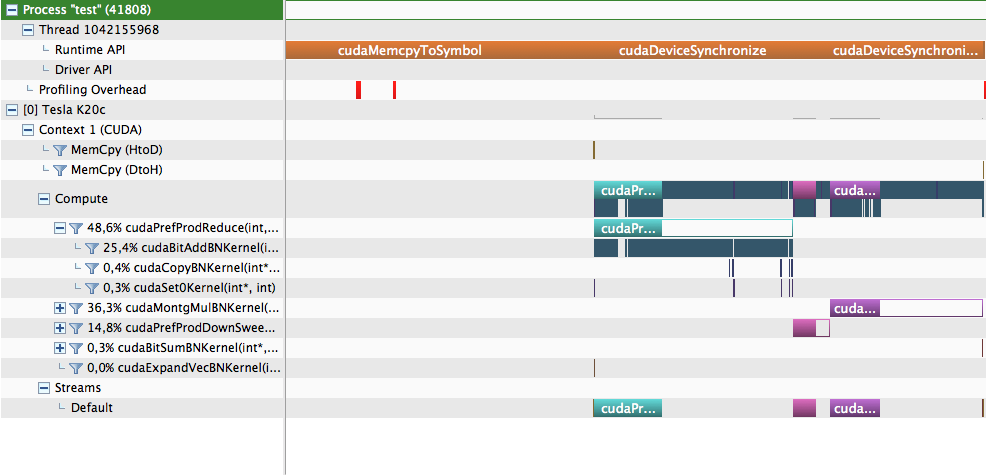
\includegraphics[scale=0.45]{Kapitel/Implementierung/cuda_timeline.png}
\caption{Profiler Analyse des Cuda Algorithmus}
\label{figure:timeline}
\end{figure}

Dieser Sachverhalt ist auch gut erkennbar, wenn man sich die prozentuale Ausführungszeit des Reduce-Steps in Abb. \ref{figure:exec_count} ansieht. Der ausgeführte Kernel ist zu fast $100\%$ inaktiv und mit der Synchronisierung der Threads beschäftigt. Es kann eventuell zu einer verbesserten Laufzeit führen wenn man versucht, die Parameter für alle zu extrahierenden Bits gesamt zu übergeben. Dadurch könnten pro Iterationsschritt alle Werte dieser Ebene für alle $x$ berechnet werden, was eventuell die Gesamtsynchronisationszeit verringert. Es könnte auch versucht werden, bei teilweise vorhandenen Werten einer Ebene den folgenden Down-Sweep-Step bereits bedingt zu starten und somit die Ausführung dieser Schritte zu überlagern. Eine optimale Lösung erfordert noch weitere Tests und auch eine durchdachte Synchronisation der einzelnen Komponenten um eine Steigerung der Laufzeit zu erreichen.

\begin{figure}
\centering
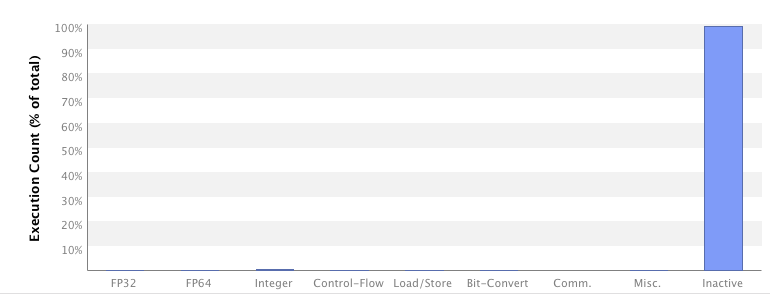
\includegraphics[scale=0.5]{Kapitel/Implementierung/cudaPrefProdReduce_execution_count.png}
\caption{Prozentuale Ausführungszeit des Reduce Steps}
\label{figure:exec_count}
Etwa $1-2\%$ der Ausführungszeit des Kernels werden für Integeroperationen verwendet. Die restliche Zeit ist der Kernel durch Synchronisierung und nicht optimale Ausnutzung der GPU inaktiv.
\end{figure}

Ein weiteres Problem ist die Speicherverwaltung im Cuda-Code. Für die verwendete Nvidia GPU K20c werden fünf verschiedene Speichertypen unterstützt, die sich alle hinsichtlich Sichtbarkeit, Zugriffsgeschwindigkeit und Größe unterscheiden

\begin{enumerate}
\item Register
	\begin{itemize}
	\item On-Chip Memory, daher sehr schnelle Zugriffszeiten
	\item Sichtbarkeit nur innerhalb eines Threads
	\item Tesla K20c: $65536$ Register pro Block
	\item Verwendete Register müssen zur Kompilierzeit feststehen
	\end{itemize}
\item Shared Memory
	\begin{itemize}
	\item On-Chip Memory, daher sehr schnelle Zugriffszeiten
	\item Sichtbarkeit nur innerhalb eines Blocks
	\item Tesla K20c: $49152$ Bytes pro Block
	\end{itemize}
\item Global Memory
	\begin{itemize}
	\item Off-Chip Memory und nicht gecached, daher langsame Zugriffszeiten
	\item Sichtbarkeit global
	\item Tesla K20c: $4800$ MBytes
	\end{itemize}
\item Local Memory
	\begin{itemize}
	\item Off-Chip Memory und nicht gecached, daher langsame Zugriffszeiten
	\item Sichtbarkeit nur innerhalb eines Threads
	\item Anhängig von Global Memory
	\end{itemize}
\item Const Memory
	\begin{itemize}
	\item Off-Chip Memory, aber gecached, daher sehr schnelle Zugriffszeiten
	\item Sichtbarkeit global
	\item Tesla K20c: $65536$ Bytes
	\end{itemize}
\end{enumerate}

Aktuell werden alle verwendeten Variablen im globalen Speicher der GPU gehalten, was zu langsamen Zugriffszeiten führt. Ein weiterer Schritt wäre zu prüfen, in wie weit der verwendetet Speicher über Shared Memory gepuffert und somit die Zugriffszeiten beschleunigt werden können. Hierbei müssen jedoch noch mehrere Dinge bedacht werden. Angenommen es wird eine Feldgröße von $1000$ Bit verwendet und jeder Threads soll lediglich sein Ergebnis puffern. Bei einer maximalen Anzahl von 1024 Threads pro Block werden insgesamt $10240000$ Bits $=$ $1280000$ Bytes benötigt, was die Größe von $49152$ Bytes pro Block bei weitem übersteigt. Passt man die Anzahl der Threads pro Block an die Größe des benötigten Shared Memory pro Thread an, reduziert sich die Anzahl der Threads pro Block auf $49$. Dadurch erhöht sich wiederum die Anzahl der benötigten Blöcke, was eine globale Synchronisierung der Blöcke unvermeidlich macht. Es muss aus diesem Grund abgewogen werden, welche Daten gepuffert werden sollen und wie sich die entstehende Anzahl der Threads pro Block auf die globale Performance auswirkt.

\subsection{Test des Cuda Algorithmus}
Getestet wurde der Cuda Algorithmus mit Hilfe von Python. Hierzu wurde die in der \textit{libtrevisan} enthaltene Funktion \textit{gen\_irreps} so erweitert, dass Python-Code generiert werden kann, der für jede Erweiterungsfeldgröße das entsprechende irreduzible Polynom zurück gibt. Der generierte Python-Code wird durch das Skript \textit{createParameterFiles.py} importiert und anschließend zwei Dateien\footnote{eine für C und eine für Python} mit folgenden Parametern erstellt:

\begin{itemize}
\item Koeffizienten
\item Anzahl der Koeffizienten
\item Größe des Erweiterungsfeldes
\item Die Stelle $x$, an der das Polynom evaluiert werden soll
\item Das irreduzible Polynom
\item Die Maske des Erweiterungsfeldes
\end{itemize}

Als Parameter müssen dem Skript \textit{createParameterFiles} die Größe des Erweiterungsfeldes, der Grad des Polynoms und die Ausgabedateien übergeben werden. Es ist somit möglich, Parameterdateien für beliebige Feldgrößen und Polynomgrade zu erstellen und den Cuda Algorithmus damit zu testen. 
Verwendet werden die Parameter zum einen in einer in C implementierten Testfunktion \textit{test.cc}, die den Cuda-Algorithmus mit diesen startet. Die Testfunktion muss mit der generierten Parameterdatei in C und dem Cuda-Code kompiliert werden. Es muss bei der Kompilierung das Präprozessor Symbols \textit{CUDA\_SANITY\_CHECKS} aktiviert sein, damit nach jedem Berechnungsschritt die Zwischenergebnisse in der Datei \textit{rsh\_test\_results} abgespeichert werden. Wenn der Cuda-Algorithmus erfolgreich beendet wurde, wird die Python-Skript \textit{analyseTestResults.py} ausgeführt und die Ergebnisse des Tests \textit{rsh\_test\_results} übergeben. Dieses Skript nutzt die für Python erstellten Parameter und führt eine Referenzimplementierung des Cuda-Algorithmus in Python aus. Anschließend werden die Ergebnisse der Referenzimplementierung mit den Resultaten in \textit{rsh\_test\_results} verglichen und alle Abweichungen ausgegeben. Der Zusammenhang zwischen den einzelnen Testschritten ist in Abb. \ref{uml:cuda_test} dargestellt.\newline

\begin{figure}
\centering
\pgfumlsdunderlinefalse
\begin{sequencediagram}
  \newthread{a}{Makefile}
  \newinst[1]{b}{gen\_irreps}
  \newinst[0.5]{c}{createParameterFiles.py}
  \newinst[0.5]{d}{test.cc}
  \newinst[0.5]{e}{analyseTestResults.py}

  \begin{call}{a}{}{b}{irreps\_cuda.py}
  \end{call}

  \begin{call}{a}{}{c}{rsh\_test\_parameters.cc/.py}
  \end{call}

  \begin{call}{a}{kompiliere Test-Code}{a}{}
  \end{call}

  \begin{call}{a}{}{d}{rsh\_test\_results}
  \end{call}

  \begin{call}{a}{}{e}{Testbericht}
  \end{call}  
\end{sequencediagram}
\caption{Zusammenhang zwischen den am Test des Cuda-Codes beteiligten Dateien}
\label{uml:cuda_test}
\end{figure}

Eine Referenzimplementierung in Python bot sich an, da Python standardmäßig Unterstützung für große Zahlen bietet und dadurch alle Algorithmen ohne Rücksicht auf Parallelisierung oder Aufspaltung der Variablen in einzelne Chunks umgesetzt werden konnten. Zudem ist Python nahezu immer auf UNIX basierten Betriebssystemen vorhanden und benötigt keine weitere Installationen zusätzlicher Compiler oder Bibliotheken. Auch die automatische Ausführung der Python Skripte gestaltete sich problemlos, da diese ohne großen Aufwand in das vorhandene Makefile eingebaut werden konnten und somit die Reihenfolge der Aufrufe und die Kompilierung des Testcodes in Abhängigkeit zur erstellten Parameterdatei kontrolliert werden konnte.\newline

Für kleine Parameter waren die Tests erfolgreich. Bei steigender Parametergröße wurde deutlich, dass der implementierte Cuda-Code noch einige Synchronisierungsprobleme aufweist, da zum Beispiel bei der Aufteilung der Threads auf mehrere Blöcke noch keine globale Synchronisierung vorhanden ist.
\section{Integration in libtrevisan}
\label{sec:integration}

\begin{figure}
\begin{lstlisting}[language=C++,captionpos=b,backgroundcolor=\color{gray!20}, caption=\"Anderungsvorschlag f"ur die Klasste \texttt{bitext}, label=lst:codevorschlag]
class bitext {
public:
	bitext(R_interp *r_interp);

	virtual ~bitext();

	void set_stat_file(const std::string &filename);

	virtual void set_input_data(void *global_rand, struct phys_params &pp);

	// Inform the bit extractor about the overlap parameter of the weak design
	virtual void set_r(long double r);

	// The following functions need to be implemented by derived
	// classes, that is, by specific 1-bit extractors.

	// Return the number of random input bits required for one
	// output bit
	virtual vertex_t num_random_bits() = 0;

	// Compute the required source entropy
	virtual uint64_t compute_k() = 0;

	// initial_rand: Pointer to randomness supplied by the weak design
	virtual bool extract(void *initial_rand) = 0;
	
	// prepare data before extraction process 
	void preExtract();
	// followUp after the extractoin process
	void postExtract();

};
\end{lstlisting}
\end{figure}
\begin{figure}
\begin{lstlisting}[language=C++,captionpos=b,backgroundcolor=\color{gray!20}, caption=\"Anderungsvorschlag f"ur Extraktionsprozess, label=lst:codevorschlag2]
// prepare extraction process
bext->preExtract();

// extract all bits, parallelism is used inside the bitext implementation
bext->extract();
	
// followUp extraction process
bext->postExtract();
\end{lstlisting}
\end{figure}

Libtrevisan ist ein in C++ implementiertes Framework, dessen Sourcecode auf GitHub\footnote{https://github.com/wolfgangmauerer/libtrevisan} verf"ugbar ist. Der Name leitet sich aus dem Ziel des Projektes ab, eine Implementierung anzubieten, die Trevisans Extraktor-Konstruktion umsetzt und leicht in eigene Projekte zu integrieren ist. Die Software wurde als Produktliniensoftware umgesetzt und ist "uber das \emph{makefile} parametrisierbar. Die Verwendung von NTL\footnote{http://www.shoup.net/ntl/} oder \emph{SSE4} kann je nach vorhandener Hard-/Software konfiguriert werden. Durch Verwendung einer Weakdesign- und einer Bitextraktor-Oberklasse, von denen konkrete Implementierungen erben, ergibt sich ein modularer Aufbau, der leicht um eigene Implementierungen erweitert werden kann.

Eine zus"atzliche Extraktorklasse "ubernimmt den Aufruf des GPU-Algorithmus. Um die GPU-Implementierung in libtrevisan zu integrieren, musste die Bibliothek an einigen Stellen angepasst werden. Die Struktur ist rein auf eine Ausf"uhrung auf der CPU ausgelegt; um mehrere CPU Kerne zu benutzen, werden mehrere Threads gestartet, die jeweils ein Bit extrahieren. Die Implementation der GPU-Variante parallelisiert jedoch die einzelne Extraktion und (noch) nicht den kompletten Vorgang. Deshalb wird, wenn erkannt wird, dass die GPU benutzt werden soll, die Anzahl der CPU Threads auf 1 begrenzt. Dar"uberhinaus ist ein h"aufiger Kontextwechsel von CPU zu GPU und umgekehrt von Nachteil, was jedoch ohne "Anderung an libtrevisan unumg"anglich w"are, da bei jedem Extraktionsschritt lokale Daten berechnet werden, die in den Speicher der GPU "ubertragen werden und, wenn ein Bit extrahiert wurde, auch r"uck"ubertragen werden. Um diesen Flaschenhals zu umgehen, werden alle im Laufe der Extraktionen ben"otigten Werte vorausberechnet, in den Speicher der GPU geschrieben und, wenn alle Bits extrahiert wurden, gesammelt zur"uck in den Hauptspeicher geschrieben. Um dies zu erm"oglichen musste die Extraktorklasse um zwei Methoden erweitert werden, wodurch der Extraktoraufruf ebenfalls angepasst werden musste, da diese Methoden nicht in der Oberklasse vorhanden sind und im normalen Extraktionsprozess nicht vorkommen. Die letzten beiden Mehtoden in Listing \ref{lst:codevorschlag} zeigen die vorgeschlagene Ver"anderung an der \texttt{bitext}-Klasse. Listing \ref{lst:codevorschlag2} skizziert den vorgeschlagenen ge"anderten Ablauf im Extraktionsprozess.

Ein zus"atzlicher Parameter im \emph{makefile} bestimmt beim "Ubersetzen von libtrevisan, ob die CUDA-Variante des RSH-Extraktors mit "ubersetzt wird oder nicht.
\section{Laufzeitanalysen}
\begin{table}[b]
	\centering
	\begin{tabular}{ll}
		\hline \hline
		\vspace{-3mm}\\
		Prozessor		& 2x Intel Xeon CPU E5-2667 0 @ 2.90GHz\\
		Arbeitsspeicher	& 8x 16 GB DDR3 @ 1600MHz\\
		Grafikkarte		& 2x Nvidia Tesla K20c\\
		Hauptplatine	& Dell 0F5XM3\\
		\hline
	\end{tabular}
	\caption{Ausstattung des Testrechners}
	\label{table:systemausstattung}
\end{table}

Das System, auf dem der Algorithmus getestet wurde, ist in Tabelle \ref{table:systemausstattung} beschrieben.

Um die Performance des Extraktors zu messen und zu vergleichen wurde ein Shellscript geschrieben. Als Testparameter wurde $m$, die Anzahl der zu extrahierenden Bits, gew"ahlt, wobei $m = 2^M$ und $M \in \{8, \dots, 20\}$. Die gew"ahlte Seedl"ange $n$ ist immer um den Faktor $16$ gr"o"ser als $m$. Um den Einfluss einzelner Ausrei"ser zu mindern, wird der Test 18 mal wiederholt. Abbildung \ref{fig:laufzeitCpuGpu2} zeigt einen Plot der Ergebnisse des Tests, wobei der Median und das obere und untere Dezil betrachtet werden.


\begin{comment}
\begin{figure}
	\centering
	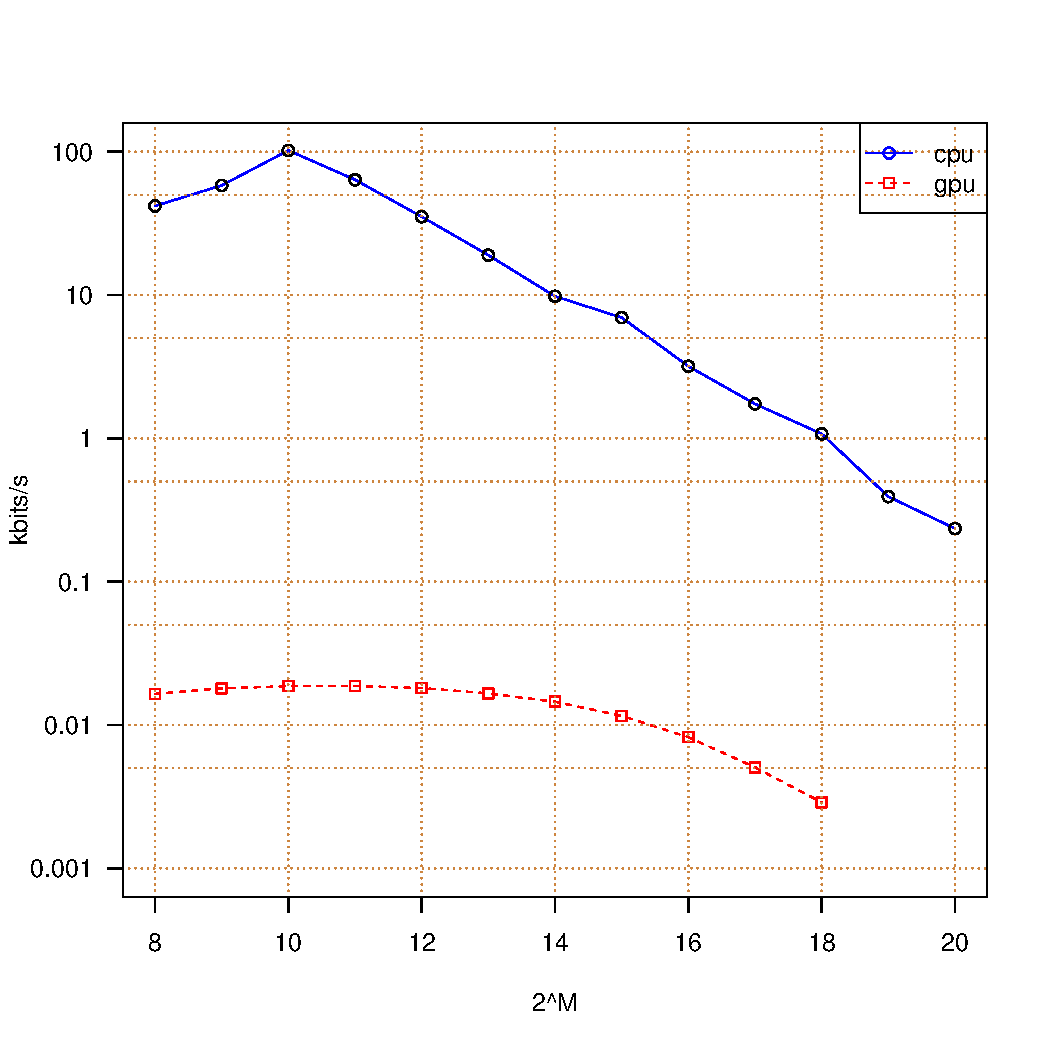
\includegraphics[scale=.5]{combined.pdf}
	\caption{Laufzeit CPU vs GPU}
	\label{fig:laufzeitCpuGpu}
\end{figure}
\end{comment}
\begin{figure}[h]
\centering
\begin{tikzpicture}[trim axis left,trim axis right]
\begin{axis} [ymode=log, xtick={8,10,12,14,16,18,20}, scale=1.5, grid=both, minor ytick={.005,.05,.5,5,50,500}, minor xtick={9,11,13,15,17,19}, legend entries={,CPU,,,,GPU},xlabel=$2^M$,ylabel={kbit/s [log. Skala]}]
    \addplot [box plot box] table {Bilder/output_rsh.dat};
    \addplot [box plot median] table {Bilder/output_rsh.dat};
    \addplot [box plot top whisker] table {Bilder/output_rsh.dat};
    \addplot [box plot bottom whisker] table {Bilder/output_rsh.dat};
    \addplot [box plot box] table {Bilder/output_rshCuda.dat};
    \addplot [box plot median, /pgfplots/other color] table {Bilder/output_rshCuda.dat};
    \addplot [box plot top whisker] table {Bilder/output_rshCuda.dat};
    \addplot [box plot bottom whisker] table {Bilder/output_rshCuda.dat};
\end{axis}
\end{tikzpicture}
\caption{Laufzeit CPU vs GPU \protect\\ \normalfont Die x-Achse des Liniendiagramms gibt die Anzahl der zu extrahierenden Bits an und \protect\\ die y-Achse zeigt die gemessene Performance in \emph{kbits/s} auf einer logarithmischen Skala.}
\label{fig:laufzeitCpuGpu2}
\end{figure}

Die beiden Testparameter $M=19$ und $M=20$ f"uhren in der aktuellen Implementierung zu Speicherzugriffsfehlern. Dies wurde w"ahrend des Entwickelns nicht deutlich, da aus Zeitgr"unden nur kleine Werte f"ur $m$ und $n$ getestet wurden (die Extraktion von $2^{18}$ Bits dauert ca. 30 Stunden).

Aus den gemessenen Werten geht hervor, dass der CPU-Algorithmus um den Faktor $10^3$ schneller ist als die GPU-Implementierung. Die Kurve des GPU-Algorithmus bleibt allerdings "uber einen gr"o"seren Wertebereich von $M$ stabil und beginnt erst bei $M=15$ vergleichbar stark abzunehmen wie der CPU-Algorithmus ab $M=10$. Da der GPU-Algorithmus einiges Potential zur Optimierung bietet, besteht die M"oglichkeit vergleichbare Extraktionsraten zu erzielen.

\section{Ausblick}



\newpage
% Verzeichnisse einbinden



%
% Literaturverzeichnis
%
\bibliography{Literaturverzeichnis/Literatur}


\end{document}